%*****************************************************************************************
%*********************************** Second Chapter **************************************
%*****************************************************************************************

 \chapter{Background}

\ifpdf
    \graphicspath{{Chapter2-Background/Figs/Raster/}{Chapter2-Background/Figs/PDF/}{Chapter2-Background/Figs/}}
\else
    \graphicspath{{Chapter2-Background/Figs/Vector/}{Chapter2-Background/Figs/}}
\fi


\section[Network Communication Paradigms]{Network Communication Paradigms}
Solutions to distributed problems are commonly associated with one of two paradigms: Synchronous and Asynchronous communication. Atomic Broadcast protocols are no exception to this rule, therefore in order to understand the challenge of designing and implementing atomic broadcast protocols, it is necessary to explore the limitations of common network paradigms.  

	\subsection{Synchronous}
	Synchronous communication refers to a communication model in which an upper bound can be placed on the communication delay experienced when sending data packets between any two nodes in the network. If a data packet exceeds this upper bound then the transmission is deemed to have failed due to a timing failure, requiring the data packet to be retransmitted. 
	
	In order to successfully calculate the upper bound on communication delays a synchronous network needs to establish an upper bound on the number of faulty nodes present in the network, the maximum load of the network and the transmission rate of data packets~\cite{Cristian:1996:SA:227210.227231}. These requirements make the synchronous paradigm unsuitable for use in middleware and distributed database systems, as such systems are typically executed on commodity hardware.  
	 
	\subsection{Asynchronous}
	The Asynchronous communication model does not define an upper bound on communication or processing delays, instead these delays are considered finite and arbitrary, resulting in the performance bounds required in the synchronous model becoming redundant. Placing no bounds on network load or the number of faulty nodes makes the asynchronous model much more flexible then the synchronous approach, enabling the asynchronous model to be implemented over various network topologies that utilise commodity hardware. 

	A limitation of the asynchronous model is the inability to distinguish between a slow or a crashed node, due to the lack of an established upper bound on communication delays.  Consequently many applications using the asynchronous models must rely on configurable timeout parameters, which can result in \emph{false suspicions}; where a slow node is incorrectly suspected of having crashed.  Conversely, it is also possible for the time outs to be too large, resulting in the system waiting longer than necessary to detect a crashed node.  
	
	\subsection{Probabilistic Synchronous}
	Recent papers have called for an alternative to the asynchronous model to be utilised when designing distributed systems. Aguilera and Walkfish~\cite{Aguilera:2009:NTA:1855568.1855571} argue that the asynchronous model is inherently unsafe. They believe that removing assumptions about synchrony at the lower layers of a system can sacrifice liveness throughout the system. Furthermore the inability to distinguish between a crash and a slow process can result in users of a system having to guess on the appropriate action to take in order to remedy the situation, potentially violating safety. 

Ezhilchelvan and Shrivastava~\cite{Ezhilchelvan:2010:LPR:1773912.1773927} introduce a new communication model, Probabilistic Synchronous Model, which aims to overcome the previously stated issues with asynchrony. The probabilistic synchronous model is based upon the assumption that, in datacentres and cluster-based environments, there is a correlation between the past and near future "performance" of the network; where performance is the probability distribution of delays. In the literature, the existence of this correlation is called stochastic patterns being stationary. The recent past performance of the network can then be used as an input parameter for distributed protocols, which utilise these values to calculate probabilistic guarantees. Monitoring the recent past performance of the network also enables protocols to utilise time outs that are considered accurate to a certain probability, enabling processes to distinguish between slow and crashed nodes. 


\section{Atomic Broadcast Protocols} \label{atomic_guarantees}
Atomic broadcast protocols, \emph{abcast} for short, are message broadcasting protocols that provide specific guarantees on message delivery to ensure that messages are delivered reliably and in the same order at all destinations.  The following guarantees must be maintained to ensure that a broadcast is atomic, with regard to the delivery order and the set of destinations that deliver the message; where delivery is the passing of a message up the network stack to a higher level protocol or application.  

\begin{itemize}
    \item [\textbf{G1}] - \emph{Validity}: If the source of $m_i$ does not crash until it \emph{abcast}s $m_i$, then all operative destinations of $m_i$ deliver $m_i$.
    \item [\textbf{G2}] - \emph{Uniform Agreement}: If the source of $m_i$ crashes while \emph{abcast}ing $m_i$, and if any destination delivers $m_i$, then all operative
destinations of $m_i$ must deliver $m_i$.
    \item [\textbf{G3}] - \emph{Uniform Integrity}: If $m_i$ has already been delivered by a destination $d$, then $d$ cannot not deliver $m_i$ again.  
    \item [\textbf{G4}] - \emph{Uniform Total Order}: If two \emph{\emph{abcast}s}, $m_i$ and $m_j$, have
common destinations, then all such destinations that deliver both $m_i$ and $m_j$, must deliver them in an identical order (i.e. $<m_i, m_j>$ or $<m_j, m_i>$)
\end{itemize}

Message delivery is a one-time, irreversible operation that occurs when a message is passed up from the \emph{abcast} protocol to the next layer in the network stack. Once a message has been delivered, it cannot be undelivered, therefore any violations of message guarantees cannot be undone at the \emph{abcast} level.  Therefore meeting G1-G4 presents two challenges, C1 and C2, that need to be met by all \emph{abcast} protocols.

Consider $m$ is to be \emph{abcast} to a set of destinations $m.dst$, where $m.dst$ contains the source of an \emph{abcast} message, as the receiving of the message incurs no additional network cost and enables the source application to receive its own message.  C1 and C2 are stated below:
\begin{itemize}
    \item[\textbf{C1}] - If an operative $d \in m.dst$ receives $m$, then every operative
     $d' \in m.dst$ must be able to receive $m$ so that G1 and G2 are not violated.
    \item[\textbf{C2}] - Every $d$ that receives $m$ must determine a \emph{safe} moment
to deliver $m$ so that G3 and G4 are not violated.
\end{itemize}

Meeting both C1 and C2 is not a trivial task, as such there is a large amount of literature\cite{Defago:2004:TOB:1041680.1041682} on \emph{abcast} protocols spanning several decades.  From the literature, it is clear that there exists two distinct approaches to solving the challenges of \emph{abcast}; \emph{Quorum based} and \emph{Group Membership} dependent protocols.  This section will describe each of these approaches and explore notable examples of each approach.  
	
    \subsection{Group Ordering}
    \emph{Abcast} protocols can provide two different types of broadcasting capability, some protocols allow messages to only be sent to a single destination set, whereas others allow messages to be sent to multiple subsets of the available destinations.  The merits of each are explored below.   
    
        \subsubsection{Single Destination Set}
        A single destination protocol is a \emph{abcast} protocol that only allows the sending of a message to one set of destinations.  For example if the total number of nodes is equal to 5, then $\left\vert{m.dst}\right\vert = 5$.
        
        Protocols that utilise a single destination set can provide performance benefits over protocols that allow multiple destination groups in scenarios where $\left\vert{m.dst}\right\vert$ is small (< 5).  This is because such protocols can piggyback additional meta information on messages as they know that the nodes in the $m.dst$ set will remain the same in the absence of node failures.  Furthermore, such protocols do not have the overhead of the overlapping subset problem described in \ref{ssec:overlapping}.  
        
        Due to $\left\vert{m.dst}\right\vert$ being equal to the number of total nodes, the scalability of single destination set protocols is underwhelming, with performance degrading dramatically as the number of nodes increase.  
        
        \subsubsection{Multiple Destination Sets}\label{ssec:overlapping}
        In contrast to single destination protocols, there a \emph{abcast} protocols that allow messages to be broadcast to multiple destination sets within the cluster.  Such protocols fall into two categories, those that only allow \emph{disjoint} sets and those that allow \emph{overlapping} sets.  
        
        The creation of disjoint \emph{abcast} protocols is trivial, as the majority of single destination set protocols can be converted into disjoint protocols with only a few minor adjustments \cite{Defago:2004:TOB:1041680.1041682}.  Disjoint protocols are not applicable to Infinispan, as the ability to only broadcast to disjoint sets of destinations does not provides a solution to either the \emph{partial} or \emph{full} replication problem, as described in \ref{sec:infinispan}.  
        
        Creating protocols that support overlapping destination sets is a challenging task, due to any node involved in two overlapping subset having to satisfy G4 for messages involved in both destination sets.  Say node $a$ broadcasts $m_i$ to $m.dst = \{a,b,c\}$ and node $d$ broadcasts $m_j$ to $m.dst = \{b,c,d\}$ the challenge is ensuring that the common destinations $\{b,c\}$ deliver both messages in the same order; either $m_i$ before $m_j$ or vice versa.  Furthermore, solving C2 becomes more difficult as we need to ensure that $\{b,c\}$ do not miss $m_i$ or $m_j$, in a way that is not overly-restrictive on performance.  
        
        
	\subsection{Group Membership based Atomic Broadcast}
	The Group Membership (GM) approach to \emph{abcast} protocols refers to a group of protocols that rely on a higher level service/protocol to maintain a current \emph{view} of nodes that are correct (not crashed).  The \emph{abcast} protocol leaves all crash detection to the GM protocol, and assumes that the latest \emph{view} $v_i$ issued by the GM protocol is representative of the network's current state.  When the GM service detects that a node has crashed, it publishes a new view $v_j$, which the \emph{abcast} protocol will utilise until a subsequent view is published.  The \emph{abcast} protocol is responsible for ensuring that guarantees G1-G4 are maintained by taking appropriate action upon receiving a new view from the GM service.  
	
	GM dependent protocols always operate on the assumption that the current view $v_i$ provided by the GM protocol is accurate.  A consequence of this is that when $v_i$ no longer represents the actual state of the network, $\left\vert v_i \right\vert \neq \left\vert ActiveNodes \right\vert$, the \emph{abcast} protocol will block severely until $v_j$ is published.  This blocking will result in a loss of availability for any \emph{abcast} messages required by higher level protocols/applications, however it is necessary to ensure that G1-G4 are maintained.  Upon receiving $v_j$, the \emph{abcast} protocol will safely remove any messages that have been received from the crashed node, but have not yet been delivered by any destination (G1).  A \emph{virtually-synchronous}\cite{Birman:1991:LCA:128738.128742} closure is typically used to ensure that all \emph{abcast} messages sent by the crashed node, that have been delivered by at least one correct destination, are delivered by all of the remaining destinations (G2).  

        \subsubsection{Newtop}
        Newtop \citep{Ezhilchelvan:1995:NFG:876885.880005} is a GM based \emph{abcast} protocol developed by Ezhilchelvan et al. that supports broadcasting to overlapping destination sets.  It utilises acknowledgements and logical clocks, to ensure that C1 and C2 are met, respectively.  
        
        To ensure that C1 is met, the delivery of a message $m$, sent by $d$, $m.o=d$, is blocked until each $d' \in m.dst-\{m.o\}$ has acknowledged $m$ by sending $ack_{d'}(m)$ to every $d \in m.dst$ and each $d \in m.dst$ has received $ack_{d'}(m) \forall m.dst \setminus \{m.o,d\}$.  This ensures that it is impossible to violate C1, as every $d$ has confirmation that $m$ has been received by all members of $m.dst$.  
        C2 is addressed by each $m$ and each $ack_{d'}(m)$ being \emph{tentatively} timestamped with a value that is one more than the timestamp ever seen or used by the respective source \cite{Lamport:1978:TCO:359545.359563}. Once $m$ and the $ack_{d'}(m)$ of every $d'\in m.dst-\{m.o\}$ are received, $d \in m.dst$ \emph{finalizes} a timestamp ($m.ts$) for $m$ as the largest of all these tentative timestamps. When $d$ delivers every received $m$ as per (finalized) $m.ts$, all guarantees are met. Proofs are in \cite{Lamport:1978:TCO:359545.359563, Birman:1991:LCA:128738.128742, Ezhilchelvan:1995:NFG:876885.880005} and the intuition is given below.
        
        Since $m.ts$ is finalized only after having received a tentative timestamp from every node in $m.dst$, for any $d \in m.dst$, $m.ts$ cannot be smaller than any of the tentative timestamps proposed for $m$, when $d$ finalizes $m.ts$, it must have received any $m'$ whose $m'.ts$ \emph{could} be finalized as $m'.ts < m.ts$. So, if $d$ finalizes $m.ts$ before finalizing $m'.ts$, it will wait for $m'.ts$ to be finalized before delivering $m$.
        
        Say, $d' \in m'.dst - \{m.o\}$ is crashed; When $d \in m'.dst$ does not receive $ack_{d'}(m')$, it is blocked from finalizing $m'.ts$ until the GM protocol confirms that $d'$ is crashed and $ack_{d'}(m')$ does not exist (through \emph{virtually synchronous} closure). Say, $d$ has proposed $ack_d(m').ts$ and also it finalizes some $m.ts$ while $d'$ remains crashed (Note: $d'$ is not in $m.dst$). If $m.ts > ack_d(m').ts$, $d$ is also blocked from delivering $m$ until $m'.ts$ is finalized, because $d$ knows that $m'.ts$ can be finalized as $m'.ts < m.ts$.

Thus, when \emph{abcast}s are initiated by an application , the longer GM takes to detect and isolate a crashed node (such as $d'$ above), the larger the number of nodes (such as $d$) that are likely to receive an \emph{abcast} (such as $m'$) whose destination set includes the crashed one and, at each such node, the larger is the number of finalized \emph{abcast}s (such as $m$) blocked from delivery.  Ultimately leading to a loss in the system's liveness.  

Although the Newtop protocol blocks severely in the presence of node crashes, in their absence it provides the smallest achievable latency available to \emph{abcast} protocols.  This is because Newtop finalises $m.ts$ within $2 \times x_{mx}$, where $x_{mx}$ is the maximum message latency between the nodes in $m.dst$.  Therefore allowing the protocol to deliver messages within $2 \times x_{mx}$ when blocking does not occur.  

Finally, if the Newtop protocol is utilised in an single destination environment, it is possible to finalise $m.ts$ and deliver messages with a single broadcast from $m.o$.  This is achieved by all $d$ piggybacking $ack_d(m)$ on subsequent messages, therefore reducing the load on the network and increasing throughput.  

	\subsection{Quorum Based Atomic Broadcast}
	Quorum based \emph{abcast} protocol are \emph{abcast} solutions that utilise a \emph{master} node to coordinate \emph{slave} nodes.  The master node is responsible for sending all messages, and proposing $m.ts$, which is confirmed when it receives $ack(m)$ from a majority of nodes; hence the name quorum-based.  Thus each \emph{abcast} requires 3 communication steps and latency can be $3 \times x_{mx}$.  
	
	The advantages of such protocols is that they preserve liveness in the presence of node failures, this is because messages can still be delivered, without blocking, when the number of slave failures is less than $\vert\vert \frac{m.dst}{2} \vert\vert - 1$.  However, mild blocking does occur when the master node is suspected of crashing, as it is necessary for a new master node to be elected before \emph{abcast} delivery can resume. Furthermore, as the master node requires a quorum of acknowledgements to proceed, it is not possible for such protocols to be utilised when $\left\vert m.dst \right\vert < 3$. 
	
	Finally, providing support for multiple destination sets in a quorum based protocol is a non-trivial task, which is beyond the scope of this thesis, therefore we will not consider it.  
		\subsubsection{Paxos}
		\subsubsection{RAFT}		
	

\section{Coordination Services}
Coordination services are centralised systems that can be utilised by distributed systems to provide commonly required services that aid process coordination. Examples of such services are: distributed lock management, low-volume storage and naming. System engineers can implement these features without using a coordination service, however these features are very complex due to their distributed nature. A coordination service hides this complexity, enabling the engineer to focus on the core functionality of their system. Furthermore, incorporating a coordination service into an existing system only requires calls to the services api, whereas, retrospectively introducing distributed services into even the simplest of systems is fraught with difficulties. 

Coordination systems are usually used by a system to store data that is crucial to their operation, therefore high availability and fault-tolerance are required. Typically, coordination services consist of a small number up of nodes (no greater than ten) that are all replicas of each other, allowing the coordination system to carry on functioning in the presence of node failures. The use of multiple nodes can also increase the number of requests that the coordination service can process simultaneously. 

In order for a coordination service to maintain replicated nodes consistently, it is necessary for a consensus to be reached when writing data to each of the replicas. Without consensus the system's data replicas would become inconsistent, which could be catastrophic for the user system's data consistency and integrity, as they could receive corrupt data from one of the inconsistent replicas. 

	\subsection{Chubby}
	Chubby ~\cite{Burrows:2006:CLS:1298455.1298487} is a distributed lock manager developed by Google that is based upon the Paxos~\cite{Lamport:1998:PP:279227.279229}~\cite{Lamport:2001:PaxosMadeSimple} consensus algorithm. Chubby cluster's typically contain five nodes, however only one node is able to service read and write requests at any one time; this node is called the master. The role of the master is to service client requests and to ensure that all write requests are executed by the replicas. Client write requests are forwarded to all data replicas using the Paxos consensus algorithm, and the request is confirmed to the client when the majority of replicas have executed the write request. 

The main advantage of the Chubby system is its focus on high availability and reliability, with production instances reported to have executed for over a year. However, the limitations of the chubby system are caused by its use of a master node. Utilising a single node to handle all read/write requests severely limits the throughput capabilities of the system because the master node will always become a bottleneck as throughput increases.  Furthermore, because Chubby utilises the Paxos consensus algorithm, the minimum number of nodes in a chubby coordination service is 3 as a quorum needs to be reached between service members.  This can be a disadvantage in systems where fast writes are required, and the use of 3 nodes for fault-tolerance is excessive.  

	\subsection{Zookeeper}
	Zookeeper ~\cite{Hunt:2010:ZWC:1855840.1855851} is an open source general purpose coordination service developed by The Apache Software Foundation. Similar to Chubby, Zookeeper also employs a master node, as it utilises the quorum-based protocol ZAB ~\cite{Junqueira:2011:ZHB:2056308.2056409} to update the data replicas.  However, unlike Chubby, in Zookeeper read requests by clients are not restricted to the master node, rather any replica node can handle them.  This is advantageous, as it reduces the number of requests that the master node has to handle, enabling the master to concentrate on maintaining a consistent state between replicas (i.e. handling write requests) and satisfying its own read requests.  
	
	Distributing read requests across the entire Zookeeper cluster mitigates the bottleneck observed in the Chubby approach, however it does not remove it as all write requests must be served by the master, thus Zookeeper favours workloads that have a read/write ratio of 10:1. Furthermore, when read requests are handled by the replica nodes it is possible for stale values to be returned to the requesting client.  This occurs if a client requests a value from a replica that has missed an \emph{abcast} by the master node, due to the replica not being involved in the quorum.  Therefore, the guarantees provided by Zookeeper can only be considered weakly-consistent.   

%\section{Transactions}

\section{In-memory Databases}
In-memory databases \citep{Infinispan, Hazelcast, GridGain} are database systems that aim to provide scalable, low-latency data storage.  Data is stored in RAM to provide fast data access, and is partitioned across multiple nodes in a cluster for scalability.  In order to provide availability and durability in the presence of node failures, each partition is replicated across distinct nodes; the number of nodes utilised is the \emph{Replication Factor} ($RF$).  Storing data in RAM provides superior read/write performance to traditional disk-based databases, whilst the distributed nature of the database allows it to elastically scale by simply adding additional nodes to store data partitions.  

The emergence of simpler NoSQL based data models, such as key/value pairs, has enabled in-memory databases to become a reality.  Previously, RDBMS services were the de facto standard for database solutions, however their rigid structure greatly limits their ability to elastically scale due to the difficulty of maintaining table structures and distributing records across multiple nodes \citep{Cattell:2011:SSN:1978915.1978919, Cooper:2010:BCS:1807128.1807152}. Distributing data across many nodes is essential for in-memory databases, not only to provide availability, but to provide sufficient storage capacity for a database system; RAM per node is typically measured in gigabytes, whereas disk based storage is measured in terabytes.  

Finally, due to RAM being a volatile storage medium (i.e its state is lost when power is lost) it is common for in-memory databases to provide a means for persistent storage in the event of power-loss or node crashes.  Typically, this is achieved through asynchronous write-requests to a persistent database that utilises the same data model as the in-memory database.  However, in some deployments, such as distributed caches, this is forsaken in order to provide applications with the lowest possible response time.  
    
    \subsection{Replication Schemes}\label{replication_schemes}
	Typically, in-memory databases offer two types of replication schemes: \emph{full} and \emph{partial} replication.  
	
	In a \emph{full} replication scheme, each data partition is replicated on every distinct node in the cluster, $RF = \left\vert nodes \right\vert$.  This greatly limits the scalability of the database, as the total number of RPCs required to update each key/value pair increases when additional nodes are added to the cluster.  Furthermore, the maximum storage capacity of the database will always be equal to the RAM size of the least capable node in the cluster.  The advantages of using \emph{full} replication is that it can provide high availability, with only a few cluster nodes, as well as providing high-performance when workloads are read dominant; full replication is extremely effective for creating highly-available distributed cache that sits between the application and a persistent database.  
	
	\emph{Partial} replication is a data scheme, where each data partition is replicated across a subset of nodes in the cluster, $RF < \left\vert nodes \right\vert$; no node holds all replicas of a given partition nor the entire database.  The advantage of this partial replication, is the total size of the database is not limited by the weakest node, rather the collective memory pool of all nodes in the cluster and the $RF$ configured by the system administrator.  Therefore, elastic scalability is possible as the database's capacity can be increased by simply adding an additional node to the cluster.  Ultimately, the scalability of a partially replicated database is determined by the size of $RF$; a high $RF$ value ($RF > 3$) will provide high levels of availability and fault-tolerance at the expense of write latency (as all $RF$ replicas need to be updated); whereas too low a value will provide low-latency writes at the expense of fault-tolerance and availability.   
	
	The total capacity of a partially replicated database can be expressed as $\frac{Mem - S.Res}{RF}$: where $Mem$ is the total amount of RAM available across the cluster, $S.Res$ is the RAM required by other system resources (operating system etc.) and $RF$ is the configured \emph{replication factor}.  

%Persistence is typically provided through asynchronous write-requests, however performance can be improved further by utilising a purely in-memory solution.  tx logs, sacrifice durability in ACID because of volatile nature

\section{Infinispan}\label{sec:infinispan}
Infinispan \citep{Infinispan} is an open-source in-memory database system developed by Red Hat, Inc \citep{RedHat}. that provides users with a JSR-107 \citep{JSR-107} compliant, key/value data model.  It can be used as a distributed cache, or as a transactional NoSQL key/value store, and supports both full and partial replication.  From its inception Infinispan has been designed  to be highly-scalable, this section describes how Infinispan has approach the challenge of implementing scalable transactions, and the limitations of some of the existing solutions.  

As previously stated ($\S$ \ref{replication_schemes}), full replication is not scalable, therefore the rest of this document will focus on the challenges posed by partial replication schemes; henceforth any reference to key/value replication assumes partial replication.  Furthermore, all references to read/write operations are assumed to be in the context of Infinispan transactions, non-transactional operations are not considered.  

    \subsection{Key Distribution}
    A key challenge of implementing distributed data stores is ensuring that each node in the cluster is aware of where each data item is located, so that it is able to access it when required.  This problem is further exasperated by Infinispan's need to elastically scale.  
    
    A naive solution is for each node in the cluster to maintain meta-data about each key/value pair stored in the database, however the maintenance of such data would create a large overhead.  Not only would the database required additional space to store the meta-data, but it would also need to update the meta-data stored on each node in the cluster every time a node was added or removed from the cluster.  Clearly this is not a scalable solution.  
    
    Infinispan solves this problem, by utilising a modified consistent hashing algorithm \citep{Karger:1997:CHR:258533.258660, Infinispan, Ruivo:2011:ETO:2120967.2121604} to determine where key/value pairs should be stored; the algorithm utilises the key as a parameter for computing the hash.  The hashing algorithm divides the cluster into segments, with each hashed key mapping to a single segment, and associates $RF$ nodes with each segment. The nodes for each segment are stored in an ordered list, with the index of a node determining its replica status.  Nodes stored at index 0 are considered the \emph{primary} owner of all keys stored in that segment, and nodes with an index greater than 0 are considered \emph{backup} owners; \emph{primary} owners are used by Infinispan to coordinate various database operations; \emph{backup} owners store data purely for fault-tolerance.  
 
    Therefore it is possible for a node to determine the \emph{primary} and \emph{backup} location of any key $k$ in the cluster, simply by calling $hash(k)$. This enables any node in the cluster to deterministically calculate the storage location of any key/value in the database without a single RPC, therefore reducing RPCs and aiding scalability.  
    
    A consequence of utilising a consistent hash function is that Infinispan users cannot specify where data should be stored in the database. This can be advantageous when the user knows that a small set of keys will commonly be read together.  In such cases, it could be beneficial to store the keys across the same range of \emph{primary} and \emph{backup} owners in order to reduce the number of RPCs required.  Infinispan circumvents this problem by allowing users to generate keys, using a modified version of the hash function, whose owners will be the same as a specified key.  
    
    \subsection{Transactions}
    %TODO? More info on optimistic and pessimistic transactions
    Unlike many NoSQL databases, Infinispan is a fully transactional data-store, with both the JTA\citep{JTA} and XA\citep{XA} standards supported.  Both optimistic \citep{Kung:1981:OMC:319566.319567} and pessimistic transactions are supported, however optimistic transactions are used in the default Infinispan configuration in order to reduce contention and the chance of deadlock.  The traditional Two Phase Commit protocol (2PC) is utilised for implementing the locking strategy in both optimistic and pessimistic transactions.  In addition to the two traditional lock based transactions, Infinispan also offers a lock-free total order transaction scheme, that relies on an atomic broadcast protocol to coordinate transactions.  
	    
    This section details the topology of Infinispan transactions, then it explores the relaxed ACID guarantees provided by Infinispan, before providing an in-depth analysis of how transactions are coordinated using locking (2PC) and lock-free (Total Order) schemes. 
    
		\subsubsection{Transaction Topology}
		For all transaction flavours offered by Infinispan, the following always applies.  A Transaction ($Tx$) is first executed locally by the transaction coordinator $Tx.c$, before a prepare $prepare(Tx)$ message is sent to all nodes $Tx.dst$ involved in $Tx$.  Only $get(k)$ operations are executed locally by $Tx.c$, and this involves sending a RPC to remote nodes if $k$ is not stored locally.  Once all $get()$ operations have been satisfied locally, the values of $k$ are appended to a $prepare(Tx)$ message that is sent to $Tx.dst$.  Each member of $Tx.dst$ then validates $Tx$ $validate(Tx)$, before committing $Tx$ $commit(Tx)$.  It is only during the $commit(Tx)$ operation that write operations are executed; write operations are only executed on nodes that host a key that is being inserted or updated.  For example if $k$ is stored on $N_1, N_2$ the operation $update(k, v)$ will only be executed by nodes $N_1, N_2$.  
		
		Note, Infinispan does offer some operations, such as \textsf{Map.put(k,v)}, that require a $get(k)$ to be executed locally by $Tx.c$ and a write operation by the host nodes, however for the sake of brevity it is assumed that all operations are exclusively read or write.  Furthermore, write operations are often executed on nodes other than the host of a key being updated so that they can be stored in a local cache in order to reduce the total number of RPCs, however this optimisation is not core to the Infinispan protocol and can be disabled, therefore this functionality is also omitted for the sake of brevity.  
    
	    \subsubsection{Relaxed ACID}
	    Infinispan transactions abide by the ACID\citep{Haerder:1983:PTD:289.291} properties, however the \emph{Consistency} and \emph{Durability} guarantees are more relaxed than those provided by traditional RDBMS transactions; Durability is relaxed as a consequence of RAM being volatile, and Consistency is relaxed in order to reduce the overhead of distributed transactions in a \emph{partially replicated} context.  
	    
		    \paragraph{Durability} \hspace{0pt} \\
		    Infinispan provides two mechanisms for providing durabilty: the first is the use of redundant key backups, i.e. the \emph{replication factor}, and the second is an optional mechanism that allows key/value pairs to be persisted to a separate persistent database.  The latter is available in two different configurations, \emph{write-through} and \emph{write-beyond}. 
		    
		    Write-through is a synchronous operation, that ensures that an insert/update operation on an Infinispan key will not complete until the value has been updated in the cache and it has been updated at the persistent store.  This ensures that the contents of the cache will always be consistent with the persistent store, therefore guaranteeing that in the event of a system wide crash all committed key/value pairs will be preserved.  The disadvantage of this approach is that the users of the cache lose the performance benefits provided by in-memory storage as any update/insert operation will always take at as long as storing the pair in a persistent store.  Ultimately, write-through is only an appropriate solution in read-heavy workloads that require a strong emphasis on durability.  
		    
		    Conversely, write-beyond offers asynchronous persistence.  Key/value updates and inserts complete as soon as the operation has completed in the cache, and the values are persisted to the persistent data store in the background using a separate thread to the users request.  This ensures that the users operation is returned as quick as possible, and low-latency is maintained, however it presents a small window in which the cache is not consistent with the persistent data store.  Therefore, it is possible for the most recent key/value write operations to be lost if all nodes containing $RF$ backups simultaneously crashed or a system wide crash occurs.  
    
	        \paragraph{Consistency} \hspace{0pt} \\ \label{consistency}
	        Infinispan does not provide support for 1-copy serialisability in its transactions, instead it provides two different isolation criteria: \emph{Read Committed (RC)} and \emph{Repeatable Read (RR)}.  
	        
	        \begin{itemize}
	            \item[\textbf{RC} -] All calls to a key $get(k)$ return the last value of $k$ committed by a transaction.  
	            \item[\textbf{RR} -] The value return by the first call to $get(k)$ will be used for all subsequent calls to $get(k)$ within the current transaction.
	        \end{itemize}   
	        
	        RC is advantageous, as it ensures that all calls to $get(k)$ always return the latest value of $k$, however each call to $get(k)$ may require a RPC, as $k$ may not be stored on the local node due to $k$ only being partially replicated across the cluster. Thus RC can be detrimental to performance in transactions that consist of multiple reads to the same key.  If such transactions are prevalent in a workload, it may be advantageous to utilise RR isolation in order to reduce the total number of RPC required by a transaction.  Infinispan implements RR by storing the value return by $get(k)$, in the transaction manager's context, and simply returns the stored value for any subsequent calls to $get(k)$.  A consequence of RR is that the potential for stale values to be utilised increases, to detect these so called \emph{write-skews}\label{write-skew} Infinispan provides an optional \emph{Write Skew Check (WSC)} for use with RR isolation.  
	        
	        The WSC determines whether a read $v = get(k)$ in a transaction $Tx$, has been invalidated by a concurrent transaction $Tx'$ committing a write $update(k, v')$ during the lifetime of $Tx$.  If $Tx'$ has performed a write on $k$ between $Tx$ performing $get(k)$ and $update(k, v+1)$, then the WSC will detect this anomaly allowing the transaction manager to abort $Tx$ so that the erroneous value $v+1$ is not committed.  

        
	    \subsubsection{Two-phase Commit Protocol}
	       The 2PC protocol is the traditional approach to coordinating distributed transactions, and as such its benefits and limitations are well understood.  Infinispan utilises the 2PC protocol for coordinating both optimistic and pessimistic transactions.  
	       
           \paragraph{Example Scenario} \label{transaction_scenario} \hspace{0pt} \\	       
           Consider the following scenario: a node $N_1$ executes a transaction $Tx$ that consists of a single write operation $update(k, v)$, however the primary and backup of $k$ are stored on $N_2$ and $N_3$ respectively, therefore it is necessary for $Tx$ to be committed at $N_1, N_2$ and $N_3$ ($Tx.dst = N_1, N_2, N_3$).  To ensure that all three nodes come to the same conclusion about the transaction, whether to commit or abort, the 2PC protocol is used.  
	       
	       \paragraph{Protocol Details} \hspace{0pt} \\
	       The 2PC is leader-based consensus algorithm that is specifically designed for coordinating distributed transactions, as the name suggests the protocol consists of two distinct phases: \emph{voting} and \emph{commit}. 
	       
	       \textbf{\emph{Voting Phase.}} The transaction coordinator $Tx.c$, ($Tx.c = N_1$) sends a $prepare(Tx)$ message to all $Tx.dst$.  Upon receiving the $prepare(Tx)$ message, all members of $Tx.dst$ will validate $validate(Tx)$ the transaction and decide whether the $Tx$ should be committed or aborted.  Once a decision has been made by a node, it sends its vote $vote(Tx)$ to $Tx.c$, and awaits further instructions.  
	       
	       \textbf{\emph{Commit Phase.}}  Once the $Tx.c$ has sent $prepare(Tx)$ to all $Tx.dst$, and has validated $Tx$, it waits to receive a $vote(Tx)$ from all $Tx.dst$.  If all $Tx.dst$ respond with a commit verdict, then $Tx.c$ sends a final commit message $commit(Tx)$ to all $Tx.dst$, and commits $Tx$ locally.  However, if $Tx.c$ receives a single vote in favour of aborting $Tx$, then $Tx$ must be aborted, so $Tx.c$ sends a abort message $abort(Tx)$ to all $Tx.dst$; $Tx.c$ does not need to wait for all $vote(Tx)$ before issuing $abort(Tx)$, instead $abort(Tx)$ is issued as soon as the first abort vote has been received.  Finally, upon receiving a $commit(Tx)$ or $abort(Tx)$ each member of $Tx.dst$ will abort or commit $Tx$ locally.  
	       
	       Figure \ref{fig:2PC} shows all of the sequences involved in 2PC based upon the example scenario, and assumes that all $Tx.dst$ vote in favour of committing $Tx$.  
	       	       
            \begin{figure}[htbp!] 
                \centering    
                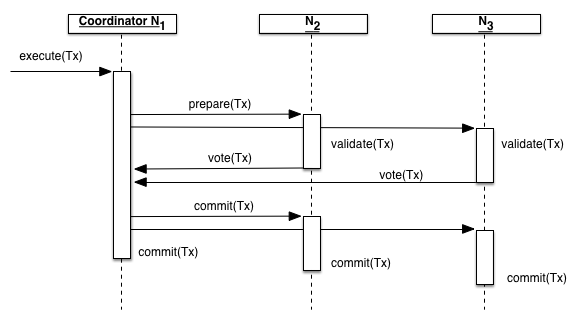
\includegraphics[width=1.0\textwidth]{2PC}
                \caption[Two-phase Commit Protocol]{2PC Sequence Diagram}
                \label{fig:2PC}
            \end{figure}
            
	        \paragraph{Key Locking} \hspace{0pt} \\
	        As previously stated, Infinispan has the notation of \emph{primary} and \emph{backup} owners of key/value pairs.  This is utilised by many functions within Infinispan, but one of the most important uses is for determining which data replica should be locked during write transactions.  Infinispan always locks the \emph{primary} owner of $k$ for write operations, never a \emph{backup}, therefore allowing each transaction to acquire a lock on $k$ at a single node.  Thus limiting the number of RPCs required to one, instead of $RF$ RPCs. For example in the previous scenario, if the \emph{primary} owner of $k$ was $N_2$, then the write lock for $k$ would only be acquired at $N_2$ instead of $N_2$ and $N_3$.  
	        
	        The time at which $k$'s lock is acquired is a defining characteristic of how transactions are handled.  Infinispan provides two different approaches, the more cautious Pessimistic transactions which utilise pessimistic locking, and Optimistic transactions that utilise optimistic locking.  Each approach is detail below along with the benefits and limitations of each approach.  
	         
            \textbf{Pessimistic Locking.}
            When pessimistic locking is used, the lock on $k$ is acquired the first time that a write operation is performed on $k$ in $Tx$ and it is held until $Tx$ either commits or aborts.  
	       		    
		    \begin{lstlisting}
		    	Tx.begin();
		    	update(k,v); // Lock is acquired
		    	Tx.commit(); // Lock is released
		    \end{lstlisting}

            This means that a RPC is issued for every write operation in the transaction, at the time the operation is encountered.  Not only does this result in an increase in network traffic, due to the number of RPCs required being equal to the number of write operations, but it also means that locks are held for a longer period of time, increasing the likelihood of deadlocks occurring.  
            
	        \textbf{Optimistic Locking.}
	        When optimistic locking\citep{Kung:1981:OMC:319566.319567} is used, the lock on $k$ is only acquired during the $prepare(Tx)$ phase of the transaction.  This means that no additional RPCs are required for locking, instead the lock is acquired by $k$'s primary when it receives $prepare(Tx)$ from $Tx.c$ and processes $Tx$ locally.  The lock is then released by $k$'s primary when $Tx$ commits or aborts.  
	        
	        Acquiring locks during the prepare phase of a transaction means that is possible for a  \emph{write-skew} ($\S$ \ref{write-skew}) to occur, therefore an optimistic transaction can be aborted due to failing the WSC (if enabled).  However, acquiring the locks during the prepare phase also reduces the total number of RPCs required by a transaction, which can improve scalability and throughput.  
	        
	        Optimistic locking is the default locking strategy employed by Infinispan, henceforth all references to lock-based transactions in Infinispan assume optimistic locking.  
	        
	        \paragraph{2PC Limitations} \hspace{0pt} \\
	        The key limitation of utilising the 2PC protocol with locking (both optimistic and pessimistic) is that it is susceptible to deadlocks.  Deadlocks occur when two concurrent transactions are trying to acquire a lock on the same set of keys.  Consider a situation where $Tx$ and $Tx'$ are executing concurrently, and both transactions want to write to key $k_1$ and $k_2$.  It is possible for $Tx$ to acquire a lock on $k_1$ with $update(k_1)$, and $Tx'$ to acquire $k_2$'s lock with $update(k_2)$.  In this scenario, it is impossible for either $Tx$ or $Tx'$ to progress as both are waiting to acquire the locks held by each other, hence deadlock.  
	        
	        Infinispan utilises timeouts in order to recover from deadlocks, with a default timeout of 10 seconds.  The transaction coordinator will wait a maximum of 10 seconds for $k$'s lock to become available, if $k$'s lock does not become available during this period, then the transaction coordinator aborts the transaction.  The limitations of this approach are that it is possible for \emph{false suspicions} to occur, as transactions can timeout due to over circumstances, such as high network load.  Furthermore, in workloads where high levels of contention are present, deadlock becomes increasingly likely, resulting in more transactions aborting, which ultimately leads to a drop in transaction throughput and Infinispan's request latency increasing.  

	    \subsubsection{Total Order Commit Protocol} \label{sec:to_commit}
	    In addition to the 2PC locking approach, Infinispan also provides a lock-free total order commit protocol, that provides the same guarantees as 2PC (\emph{Read Committed}, or \emph{ Read Repeatable}) without locking key/values during write operations.  
	    
	    The key benefit of a total order commit, is that it does not utilise locks to ensure ACIDity.  Instead it utilises the guarantees (G1-G4 $\S$ \ref{atomic_guarantees}) provided by \emph{abcast} protocols to ensure that transactions are processed sequentially and in the same total order at all destinations.  The absence of locks, removes the potential for distributed deadlocks, which reduces the total number of aborting transactions, therefore increasing transaction throughput\citep{Ruivo:2011:ETO:2120967.2121604}.  Furthermore, the use of total order commit allows transactions to be committed in only one phase (1PC) when RC or RC consistency ($\S$ \ref{consistency}) is used.  
	    
	        \paragraph{One-phase Commit} \hspace{0pt} \\
	        Consider the scenario in \ref{transaction_scenario}.  The transaction coordinator $Tx.c$, ($Tx.c = N_1$), executes the transaction locally (i.e. all $get(k)$ operations are resolved) and sends $prepare(Tx)$ using an atomic broadcast protocol to $Tx.dst$.  Because $prepare(Tx)$ is sent to $Tx.dst$ using an \emph{abcast} protocol, we can guarantee that all $Tx.dst$ will receive $prepare(Tx)$ in the same total order.  Therefore, if RR or RC is used each transaction can be committed as soon as it is received by a node without violating Infinispan's ACID properties.  Figure \ref{fig:total_order_1PC} , below, shows the sequences involved in a 1PC transaction.  
	        
            \begin{figure}[htbp!] 
                \centering    
                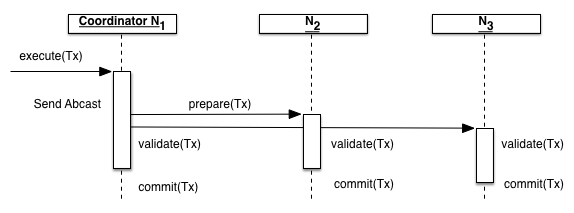
\includegraphics[width=1.0\textwidth]{1PC-Abcast}
                \caption[Total Order One-phase Commit Protocol]{Total Order 1PC Sequence Diagram}
                \label{fig:total_order_1PC}
            \end{figure}	        
	        
		        
			\paragraph{Two-phase with WSC} \hspace{0pt} \\        
	        If RR is utilised with WSC enabled, the total order commit becomes a two-phase protocol.  The first phase is the same as above, with $Tx.c$ sending $prepare(Tx)$ to all $Tx.dst$ using an \emph{abcast} protocol, however it is not possible to commit the transaction instantly, instead an additional voting stage is required.  All $Tx.dst$ validate the transaction based upon the WSC criteria and decide whether the transaction should be committed or aborted, this vote $vote(Tx)$ is then sent to $Tx.c$.  The $Tx.c$ waits to receive a $vote(Tx)$ from all $Tx.dst$, before sending a $commit(Tx)$ or $abort(Tx)$ to all $Tx.dst$.  Finally, upon receiving a $commit(Tx)$ or $abort(Tx)$ each member of $Tx.dst$ will abort or commit $Tx$ locally.          
	        
			The overhead of this additional phase is slightly reduced by two minor optimisations.  First, the $Tx.c$ does not have to receive a vote from all nodes hosting a key replica, just one, as the processing of a transaction is deterministic it is guaranteed that all replicas reach the same conclusion during WSC validation.  Secondly, like 2PC, as soon as a single $abort(Tx)$ vote is received by $Tx.c$ the transaction is aborted.  
			
			Figure \ref{fig:total_order_wsc} shows the sequences involved in a transaction that utilises the WSC.  In this figure we have assumed that $Tx.c$ receives $vote(Tx)$ from both $N_2$ and $N_3$ before sending $commit(Tx)$, however, as stated above, this is not essential, and it is valid for $Tx.c$ to have only received $vote(Tx)$ from $N_2$ or $N_3$ before sending $commit(Tx)$.  
	        
	        \begin{figure}[htbp!] 
                \centering    
                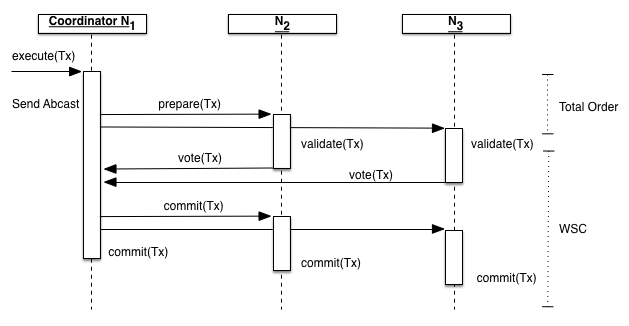
\includegraphics[width=1.0\textwidth]{WSC-Abcast}
                \caption[Total Order Commit with Write Skew Check]{Total Order with WSC Sequence Diagram}
                \label{fig:total_order_wsc}
            \end{figure}	      	
                        
	        \subsubsection{Total Order Anycast - Atomic Broadcast Protocol}
	        Total Order Anycast (TOA)\cite{Ruivo:2011:ETO:2120967.2121604} is the \emph{abcast} protocol currently utilised by Infinispan for coordinating Total Order transactions (\ref{sec:to_commit}).  It is a GM dependent protocol that, like Newtop\citep{Ezhilchelvan:1995:NFG:876885.880005}, utilises logical clocks and acknowledgements, to solve C1 and C2 (\ref{atomic_guarantees}) respectively.  
	        
			TOA's structure is very similar to the 2PC protocol, in that it consists of two distinct phases, both of which are required for a message $m$ to be delivered.  The \emph{ack phase} requires that all destinations in $m.dst$ acknowledge the message origin $m.o$, and the \emph{delivery phase} involves $m.o$ instructing all $m.dst$ to deliver $m$.  Thus the ack and delivery phases are the equivalent of the \emph{vote} and \emph{commit} phases, respectively.  
	        
			The ack phase consists of all $d' \in m.dst-\{m.o\}$ acknowledging $m$ by sending $ack_{d'}(m)$ to $m.o$.  Once $m.o$ has received all $ack_{d'}(m)$, the ack phase is complete, and C1 is guaranteed as all $m.dst$ are known to have received $m$.  
			
			The delivery phase is necessary so that all $m.dst$ know the final total order of $m$.  As in Newtop, TOA ensures C2 by piggybacking the timestamp of a logical clock onto all $m$, $ack(m)$ and $deliver(m)$ messages.  However, in TOA the timestamp of $m$ is always finalised by $m.o$ after the ack phase has completed, with the $deliver(m)$ message containing the final timestamp of $m$ in order to dictate the $m$'s total order to all $m.dst$.  
			
			The advantage of utilising $m.o$ as a central coordinator, opposed to all $m.dst$ acknowledging each other, is that the total number of messages involved in a single \emph{abcast} is reduced as $\left\vert m.dst \right\vert$ increases.  The total remote message cost for TOA and Newtop is expressed below:
			
			\begin{equation*}
		     \begin{aligned}
		       x &= \left\vert m.dst-\{m.o\} \right\vert \\
		       TOA & = 3x \\
		       Newtop & = x + x^2
		     \end{aligned}
		    \end{equation*}

	        \paragraph{TOA Limitations} \hspace{0pt} \\
			The TOA protocol suffers from the same limitations as other GM based protocols, most notably that message delivery is blocked severely in the presence of node failures.  In the context of Infinispan total order transactions, a crashed node $c$ will cause all transactions that interact with $c$ to block until the GM service issues a new view.  This causes the \emph{liveness} of all nodes interacting with $c$ to be lost in the interim period, as the blocked transactions will not be able to commit, resulting in a loss of throughput.  
	        
	        Another limitation of the TOA protocol is that it does not scale well as the number of destinations $N$ increase.  All broadcast protocols incur $1->N$ communication (i.e. $m.o$ broadcasting $m$ to all $m.dst$) as it is necessary for each destination to receive $m$.  However, $N->1$ communication (i.e. $N$ destinations in $m.dst$ sending an acknowledgment to $m.o$) is expensive, as the total time taken is equal to the slowest $N$.  Therefore, any protocol that relies on $N->1$ communication is more liable to encounter slow or crashed nodes as $N$ increases, and is ultimately more likely to block.  This means that as the number of operations in a transaction increase and keys become more distributed, the latency involved in each transaction will also increase, severely hampering Infinispan's ability to scale elastically.  
	        


%\section{RMSys}
%RMSys is a probabilistic broadcast protocol developed by Ezhilchelvan et al.~\cite{rmsys} that utilises the probabilistic synchronous model. It aims to provide the application with probabilistic guarantees on end-to-end message delivery and latency. These guarantees are calculated by RMSys’s Evaluation Component (EC) based upon the recent performance of the network and the requirements of the application. The recent performance of the network is periodically assessed by the Network Measurement Component (NMC) in order to build a Cumulative Distribution Function (CDF) of message latencies. This CDF is delivered to the EC, which uses this data to calculate the probabilistic guarantees that are delivered to the application.  
%
%Initial experiments with RMSys provided encouraging results: (i) stationary assumption holds, and (ii) timeliness and reliability can be close to probability 1. These results, and the benefits of using the probabilistic synchronous model, convinced us that RMSys was a suitable foundation for our atomic broadcast solution. 